\section{Diferenciales Exactas}

\begin{ejercicio} \label{ej:3.1}
    Calcula, si es posible, una función potencial para las siguientes parejas de funciones. Especifica en cada caso el
    dominio en el que se trabaja.
    \begin{enumerate}
        \item $P(x, y) = x + y^3$, $Q(x, y) = \nicefrac{x^2}{2} + y^2$.
        
        En este caso, $\Omega=\bb{R}^2$, que trivialmente es convexo y por tanto estrellado. Además, $P,Q\in C^1(\Omega)$ al ser polinomios. Veamos ahora si se cumple la condición de exactitud:
        \begin{equation*}
            \frac{\partial P}{\partial y}(x,y) = 3y^2 \qquad
            \frac{\partial Q}{\partial x}(x,y)= x
        \end{equation*}

        Por tanto, como no se tiene que $\frac{\partial P}{\partial y}(x,y)=\frac{\partial Q}{\partial x}(x,y)$ para todo $(x,y)\in\Omega$, no se da la condición de exactitud y no existe por tanto una función potencial para el campo vectorial $(P,Q)$.
        \item $P(x, y) = \nicefrac{1}{2} \sen 2x - xy^2$, $Q(x, y) = y(1 - x^2)$
        
        En este caso, $\Omega=\bb{R}^2$, que trivialmente es convexo y por tanto estrellado. Además, $P,Q\in C^1(\Omega)$ al ser composición, suma y producto de funciones de clase $1$. Veamos ahora si se cumple la condición de exactitud:
        \begin{equation*}
            \frac{\partial P}{\partial y}(x,y) = -2xy = \frac{\partial Q}{\partial x}(x,y)
        \end{equation*}

        Por tanto, existe una función potencial para este campo vectorial. Para encontrarla, como se busca que $\dfrac{\partial U}{\partial y}=Q$, tenemos que:
        \begin{equation*}
            U(x,y)=\int Q(x,y)dy =
            \int y(1-x^2)dy = \frac{y^2}{2}(1-x^2)+\varphi(x)
        \end{equation*}
        donde $\varphi:\bb{R}\to\bb{R}$ es una función que depende solo de $x$ y representa la constante de integración. Derivando $U$ respecto de $x$ obtenemos:
        \begin{align*}
            \frac{\partial U}{\partial x}(x,y)&=\frac{-2xy^2}{2}+\varphi'(x)\\
            \frac{\partial U}{\partial x}(x,y)&=P(x,y)=-xy^2+\nicefrac{1}{2}\sen 2x
        \end{align*}

        Por tanto, $\varphi'(x)=\nicefrac{1}{2}\sen 2x$. Entonces (y eligiendo como constante de integración $0$ por ser el potencial único salvo una constante aditiva):
        \begin{equation*}
            \varphi(x)=\int \frac{1}{2}\sen 2xdx=-\frac{1}{4}\cos 2x
        \end{equation*}

        Por tanto, la función potencial es (salvo una constante aditiva):
        \begin{equation*}
            U(x,y)=\frac{y^2}{2}(1-x^2)-\frac{1}{4}\cos 2x
        \end{equation*}

        \item \label{ej:3.1c} $P(x, y) = \sqrt{x+y}+\sqrt{x-y}$, $Q(x, y) = \sqrt{x+y}-\sqrt{x-y}$.
        
        Estudiemos en este caso el dominio $\Omega$, que no es trivial. Para que $P,Q\in C^1(\Omega)$, necesitamos que:
        \begin{equation*}
            \Omega=\{(x,y)\in\bb{R}^2 \mid x> y\}\cap\{(x,y)\in\bb{R}^2 \mid x> -y\}
            = \{(x,y)\in\bb{R}^2 \mid x>0, -x< y< x\}
        \end{equation*}

        Representamos el dominio en la Figura~\ref{fig:3.1c}.
        \begin{figure}[h]
            \centering
            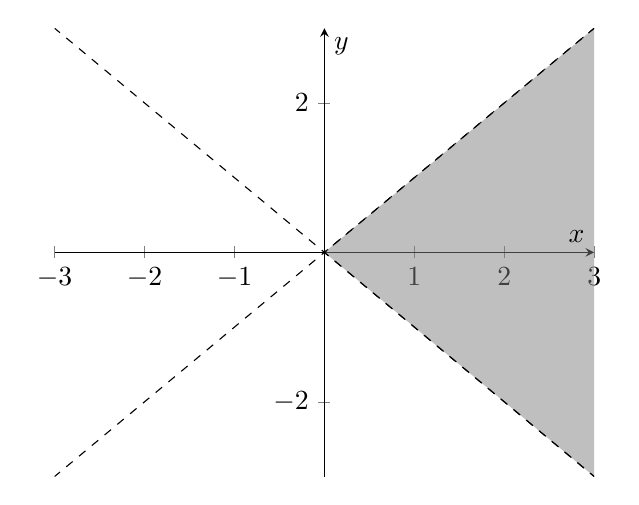
\begin{tikzpicture}
                \begin{axis}[
                    axis lines = center,
                    xlabel = \(x\),
                    ylabel = \(y\),
                    xmin = -3, xmax = 3,
                    ymin = -3, ymax = 3,
                ]
                
                \addplot [samples=2, dashed] {x};
                \addplot [samples=2, dashed] {-x};
    
                % Triangulo (4,4) (0,0) (4,-4)
                \addplot [fill=gray, fill opacity=0.5, dashed] coordinates {(4,4) (0,0) (4,-4)};
                \end{axis}
            \end{tikzpicture}
            \caption{Dominio $\Omega$ del Ejercicio~\ref{ej:3.1}.\ref{ej:3.1c}.}
            \label{fig:3.1c}
        \end{figure}

        Veamos ahora que $\Omega$ es convexo y por tanto estrellado, algo que intuitivamente podemos deducir.
        \begin{itemize}
            \item Sean $z=(x,y),~z'=(x',y')\in\Omega$, y veamos que $[z,z']\subset\Omega$.
            \begin{align*}
                [z,z']&=\{t(x,y)+(1-t)(x',y')\mid t\in[0,1]\}
                =\\&= \{(tx+(1-t)x',ty+(1-t)y')\mid t\in[0,1]\}
            \end{align*}
            \begin{itemize}
                \item Por un lado, como $x,x'>0$ y $t,1-t\geq 0$ pero no se anulan a la vez, tenemos que $tx+(1-t)x'>0$.
                \item Por otro lado, sabiendo que $-x<y<x$ y $-x'<y'<x'$, razonamos de forma directa que:
                \begin{equation*}
                    -(tx+(1-t)x')=t(-x)+(1-t)(-x')<ty+(1-t)y'<tx+(1-t)x'
                \end{equation*}
            \end{itemize}
            Por tanto, $[z,z']\subset\Omega$ y $\Omega$ es convexo.
        \end{itemize}

        Además, como los argumentos de las raíces son positivos, $P,Q\in C^1(\Omega)$. Veamos ahora si se cumple la condición de exactitud:
        \begin{align*}
            \frac{\partial P}{\partial y}(x,y) &= \frac{1}{2\sqrt{x+y}}-\frac{1}{2\sqrt{x-y}} = \frac{\partial Q}{\partial x}(x,y)
        \end{align*}

        Por tanto, existe una función potencial para este campo vectorial. Para encontrarla, como se busca que $\dfrac{\partial U}{\partial x}=P$, tenemos que:
        \begin{equation*}
            U(x,y)=\int P(x,y)dx =
            \int \sqrt{x+y}+\sqrt{x-y}dx = \frac{2}{3}(x+y)^{\nicefrac{3}{2}}+\frac{2}{3}(x-y)^{\nicefrac{3}{2}}+\varphi(y)
        \end{equation*}
        donde $\varphi:\bb{R}\to\bb{R}$ es una función que depende solo de $y$ y representa la constante de integración. Derivando $U$ respecto de $y$ obtenemos:
        \begin{align*}
            \frac{\partial U}{\partial y}(x,y)&=\sqrt{x+y}-\sqrt{x-y}+\varphi'(y) \\
            \frac{\partial U}{\partial y}(x,y)&=Q(x,y)=\sqrt{x+y}-\sqrt{x-y}
        \end{align*}

        Por tanto, $\varphi'(y)=0$. Entonces, por ejemplo, $\varphi(y)=0$. Por tanto, la función potencial es (salvo una constante aditiva):
        \begin{equation*}
            U(x,y)=\frac{2}{3}(x+y)^{\nicefrac{3}{2}}+\frac{2}{3}(x-y)^{\nicefrac{3}{2}}
        \end{equation*}
    \end{enumerate}
\end{ejercicio}

\begin{ejercicio}
    Resuelve las siguientes ecuaciones, sabiendo que admiten un factor integrante que depende de una sola de las
    variables $x$, $y$.
    \begin{enumerate}
        \item $6xy + (4y + 9x^2)y' = 0$
        
        El dominio de esta ecuación es $D=\bb{R}^2$, que es abierto y conexo. Buscamos obtener un factor integrante $\mu:\Omega \to\bb{R}$, donde $\Omega$ será el dominio del factor integrante que más adelante daremos. Para ello, necesitamos que se cumpla la condición de exactitud tras multiplicar por $\mu$. Definimos:
        \Func{P}{\bb{R}^2}{\bb{R}}{(x,y)}{6xy}
        \Func{Q}{\bb{R}^2}{\bb{R}}{(x,y)}{4y+9x^2}

        Tenemos $P,Q\in C^1(\bb{R}^2)$ por ser polinómicas. Calculemos las derivadas parciales implicadas en la condición de exactitud:
        \begin{align*}
            \frac{\partial (\mu P)}{\partial y} &= \dfrac{\partial \mu}{\partial y}P+\mu\dfrac{\partial P}{\partial y}\\
            \frac{\partial (\mu Q)}{\partial x} &= \dfrac{\partial \mu}{\partial x}Q+\mu\dfrac{\partial Q}{\partial x}
        \end{align*}

        Por tanto, la condición de exactitud se traduce en:
        \begin{equation*}
            \dfrac{\partial \mu}{\partial y}P- \dfrac{\partial \mu}{\partial x}Q = \mu\left(\dfrac{\partial Q}{\partial x}-\dfrac{\partial P}{\partial y}\right)
        \end{equation*}

        Comprobemos ahora que admite un factor integrante que depende solo de $y$. Sea $m:\pi_2(\Omega)\to \bb{R}$ de forma que $\mu(x,y)=m(y)$ para todo $(x,y)\in\Omega$. Entonces, tenemos que las derivadas parciales de $\mu$ son:
        \begin{equation*}
            \dfrac{\partial \mu}{\partial x}(x,y)=0 \qquad \dfrac{\partial \mu}{\partial y}(x,y)=m'(y)\qquad \forall (x,y)\in\Omega
        \end{equation*}

        Por tanto, la condición de exactitud se traduce en:
        \begin{align*}
            m'(y)\cdot 6xy &= m(y)\left(18x-6x\right) \qquad \forall (x,y)\in\Omega\\
            m'(y)\cdot y &= m(y)\cdot 2
        \end{align*}

        Para obtener el factor integrante $m$, planteamos la siguiente ecuación diferencial donde, como $m(y)\neq 0$ para todo $y\in\pi_2(\Omega)$, suponemos que $m(y)>0$ (en caso contrario, habríamos obtenido otro factor integrante válido):
        \begin{equation*}
            m'=\frac{2}{y}m \qquad \text{con dominio }\left\{
                \begin{array}{c}
                    \bb{R}^+\times \bb{R}^+\\
                    \lor\\
                    \bb{R}^-\times \bb{R}^+
                \end{array}
            \right.
        \end{equation*}
        Esta es una ecuación en variables separadas sin soluciones constantes, luego:
        \begin{align*}
            \int \frac{dm}{m} = \int \frac{2}{y}dy
            \Longrightarrow \ln (m) = 2\ln |y|
            \Longrightarrow m(y) = |y|^2 = y^2
        \end{align*}
        donde he supuesto constante aditiva nula (ya que tan solo buscamos un factor integrante). Por tanto, un factor integrante es $\mu(x,y)=y^2$ para todo $(x,y)\in\Omega$, donde hay dos posibles dominios:
        \begin{equation*}
            \Omega=\left\{
                \begin{array}{rcl}
                    \Omega_+ &=& \bb{R} \times \bb{R}^+\\
                    &\lor&\\
                    \Omega_- &=& \bb{R} \times \bb{R}^-
                \end{array}
            \right.
        \end{equation*}
        En cualquiera de los casos, $\Omega$ es abierto, conexo y estrellado, con $P,Q\in C^1(\Omega)$. Consideramos la siguiente ecuación diferencial:
        \begin{equation*}
            \mu P + \mu Q y' = 0 \qquad \text{con dominio }\Omega
        \end{equation*}

        Hemos visto que esa ecuación cumple la condición de exactitud. Buscamos ahora el potencial $U:\Omega\to\bb{R}$ tal que $\nabla U=(\mu P,\mu Q)$. Usando la derivada parcial respecto de $x$, tenemos que:
        \begin{equation*}
            U(x,y)=\int \mu P dx = \int 6xy\cdot y^2 dx = 6y^3\int x dx = 3y^3x^2 +\varphi(y)
        \end{equation*}
        donde $\varphi:\pi_2(\Omega)\to\bb{R}$ es una función que depende solo de $y$ y representa la constante de integración. Derivando $U$ respecto de $y$ obtenemos:
        \begin{align*}
            \frac{\partial U}{\partial y}(x,y)&=9y^2x^2+\varphi'(y)\\
            \frac{\partial U}{\partial y}(x,y)&=\mu Q(x,y)=y^2(4y+9x^2)=9y^2x^2+4y^3
        \end{align*}

        Por tanto, $\varphi'(y)=4y^3$. Entonces, por ejemplo, $\varphi(y)=y^4$. Por tanto, la función potencial es (salvo una constante aditiva):
        \begin{equation*}
            U(x,y)=3y^3x^2+y^4\qquad \forall (x,y)\in\Omega
        \end{equation*}

        Por tanto, tenemos que:
        \begin{equation*}
            0=\mu(x,y)\cdot (P(x,y)+Q(x,y)y')=\dfrac{d}{dx}\left(U(x,y)\right)=0\qquad \forall (x,y)\in\Omega
        \end{equation*}

        Veamos ahora qué valores anulan a $Q$:
        \begin{equation*}
            Q(x,y)=0 \Longleftrightarrow
            4y + 9x^2 = 0 \Longleftrightarrow y=-\frac{9}{4}x^2
        \end{equation*}

        Por tanto, para cada $(x_0, y_0)\in \Omega$ tal que $y_0\neq \nicefrac{-9}{4}x_0^2$, tenemos que la ecuación $U(x,y)=U(x_0,y_0)$ define una función implícita $y(x)$ en un entorno de $x_0$, que es solución de la ecuación diferencial de partida.

        \item $2y \cos x - xy \sen x + (2x \cos x)y' = 0$
        
        El dominio de esta ecuación es $D=\bb{R}^2$, que es abierto y conexo. Buscamos obtener un factor integrante $\mu:\Omega \to\bb{R}$, donde $\Omega$ será el dominio del factor integrante que más adelante daremos. Para ello, necesitamos que se cumpla la condición de exactitud tras multiplicar por $\mu$. Definimos:
        \Func{P}{\bb{R}^2}{\bb{R}}{(x,y)}{2y \cos x - xy \sen x}
        \Func{Q}{\bb{R}^2}{\bb{R}}{(x,y)}{2x \cos x}

        Tenemos $P,Q\in C^1(\bb{R}^2)$ por ser composición, suma y producto de funciones de clase $1$. Calculemos las derivadas parciales implicadas en la condición de exactitud:
        \begin{align*}
            \frac{\partial (\mu P)}{\partial y} &= \dfrac{\partial \mu}{\partial y}P+\mu\dfrac{\partial P}{\partial y}\\
            \frac{\partial (\mu Q)}{\partial x} &= \dfrac{\partial \mu}{\partial x}Q+\mu\dfrac{\partial Q}{\partial x}
        \end{align*}

        Por tanto, la condición de exactitud se traduce en:
        \begin{equation*}
            \dfrac{\partial \mu}{\partial y}P- \dfrac{\partial \mu}{\partial x}Q = \mu\left(\dfrac{\partial Q}{\partial x}-\dfrac{\partial P}{\partial y}\right)
        \end{equation*}

        Calculamos ahora las deriavadas parciales de $Q,P$ que nos faltan:
        \begin{equation*}
            \left\{
                \begin{aligned}
                    \frac{\partial P}{\partial y}(x,y) &= 2\cos x - x\sen x\\
                    \frac{\partial Q}{\partial x}(x,y) &= 2\cos x - 2x\sen x
                \end{aligned}
            \right\}
            \Longrightarrow
            \dfrac{\partial Q}{\partial x}-\dfrac{\partial P}{\partial y} = x\sen x
        \end{equation*}

        Por tanto, comprobemos que admite un factor integrante que depende solo de $x$. Sea $m:\pi_1(\Omega)\to \bb{R}$ de forma que $\mu(x,y)=m(x)$ para todo $(x,y)\in\Omega$. Entonces, tenemos que las derivadas parciales de $\mu$ son:
        \begin{equation*}
            \dfrac{\partial \mu}{\partial x}(x,y)=m'(x)\qquad \dfrac{\partial \mu}{\partial y}(x,y)=0\qquad \forall (x,y)\in\Omega
        \end{equation*}

        Por tanto, la condición de exactitud se traduce en:
        \begin{equation*}
            m'(x)\cdot (2x\cos x) = m(x)\cdot x\sen x \qquad \forall (x,y)\in\Omega
        \end{equation*}

        Para obtener el factor integrante $m$, planteamos la siguiente ecuación diferencial donde, como $m(x)\neq 0$ para todo $x\in\pi_1(\Omega)$, suponemos que $m(x)>0$ (en caso contrario, habríamos obtenido otro factor integrante válido):
        \begin{equation*}
            m'=\dfrac{x\sen x}{2x\cos x} m
            = \dfrac{\tg(x)}{2}\cdot m            
            \qquad \text{con dominio } \left]0,\nicefrac{\pi}{2}\right[\times \bb{R}^+
        \end{equation*}
        donde hemos elegido ese dominio por ser una de las componentes conexas del dominio de la rama principal de la función tangente. Se podrían elegir otros dominios, pero dependería de la condición inicial. Esta es una ecuación en variables separadas sin soluciones constantes, luego:
        \begin{align*}
            \int \frac{dm}{m} = \int \frac{\tg(x)}{2}dx
            \Longrightarrow \ln (m) = -\frac{1}{2}\ln (\cos x)
            \Longrightarrow m(x) = \frac{1}{\sqrt{\cos x}}
        \end{align*}
        donde he supuesto constante aditiva nula (ya que tan solo buscamos un factor integrante). Por tanto, un factor integrante es $\mu(x,y)=\dfrac{1}{\sqrt{\cos x}}$ para todo $(x,y)\in\Omega$, donde un posible dominio (de nuevo, dependería de la condición inicial) es:
        \begin{equation*}
            \Omega=\left]0,\nicefrac{\pi}{2}\right[\times \bb{R}
        \end{equation*}

        En cualquiera de los casos, $\Omega$ es abierto, conexo y estrellado, con $P,Q\in C^1(\Omega)$. Consideramos la siguiente ecuación diferencial:
        \begin{equation*}
            \mu P + \mu Q y' = 0 \qquad \text{con dominio }\Omega
        \end{equation*}

        Hemos visto que esa ecuación cumple la condición de exactitud. Buscamos ahora el potencial $U:\Omega\to\bb{R}$ tal que $\nabla U=(\mu P,\mu Q)$. Usando la derivada parcial respecto de $y$, tenemos que:
        \begin{equation*}
            U(x,y)=\int \mu Q dy = \int 2x\cos x\cdot \dfrac{1}{\sqrt{\cos x}} dy = 2xy\sqrt{\cos x}+\varphi(x)
        \end{equation*}
        donde $\varphi:\pi_1(\Omega)\to\bb{R}$ es una función que depende solo de $x$ y representa la constante de integración. Derivando $U$ respecto de $x$ obtenemos:
        \begin{align*}
            \frac{\partial U}{\partial x}(x,y)&=2y\left(\sqrt{\cos x}-\dfrac{x\sen x}{2\sqrt{\cos x}}\right)+\varphi'(x)\\
            \frac{\partial U}{\partial x}(x,y)&=\mu P(x,y)=\dfrac{1}{\sqrt{\cos x}}\left(2y\cos x - xy\sen x\right)
        \end{align*}

        Por tanto, tenemos que $\varphi'(x)=0$. Entonces, por ejemplo, $\varphi(x)=0$. Por tanto, la función potencial es (salvo una constante aditiva):
        \begin{equation*}
            U(x,y)=2xy\sqrt{\cos x}\qquad \forall (x,y)\in\Omega
        \end{equation*}

        Por tanto, tenemos que:
        \begin{equation*}
            0=\mu(x,y)\cdot (P(x,y)+Q(x,y)y')=\dfrac{d}{dx}\left(U(x,y)\right)=0\qquad \forall (x,y)\in\Omega
        \end{equation*}

        Veamos ahora qué valores anulan a $Q$:
        \begin{equation*}
            Q(x,y)=0 \Longleftrightarrow
            2x \cos x
        \end{equation*}

        No obstante, como en nuestro dominio no se puede anular la función $\tan x$, no hay valores que anulen a $Q$ en $\Omega$. Por tanto, para cada $(x_0, y_0)\in \Omega$, tenemos que la ecuación $U(x,y)=U(x_0,y_0)$ define una función implícita $y(x)$ en un entorno de $x_0$, que es solución de la ecuación diferencial de partida.       

    \end{enumerate}
\end{ejercicio}

\begin{ejercicio}
    Encuentra $p$, $q \in \bb{R}$ para que la ecuación
    \[
        -y^2 + (x^2 + xy)y' = 0
    \]
    admita un factor integrante de la forma $\mu(x, y) = x^p y^q$. Usa dicho factor integrante para resolver la ecuación. Indica un método de resolución alternativo.\\

    Para que la ecuación admita un factor integrante de la forma $\mu(x, y) = x^p y^q$, necesitamos que se cumpla la condición de exactitud tras multiplicar por $\mu$. Definimos:
    \Func{P}{\bb{R}^2}{\bb{R}}{(x,y)}{-y^2}
    \Func{Q}{\bb{R}^2}{\bb{R}}{(x,y)}{x^2+xy}

    Por tanto, tenemos que:
    \begin{align*}
        \mu(x,y) P(x,y)&=x^p y^q\cdot (-y^2)=-x^p y^{q+2}\\
        \mu(x,y) Q(x,y)&=x^p y^q\cdot (x^2+xy)=x^{p+1}y^q(x+y)
    \end{align*}

    Tenemos $P,Q\in C^1(\bb{R}^2)$ por ser polinómicas. Impongamos ahora que se cumpla la condición de exactitud:
    \begin{align*}
        \frac{\partial (\mu P)}{\partial y}(x,y) &= -(q+2)x^p y^{q+1}=x^py^q(-(q+2)y)\\
        \frac{\partial (\mu Q)}{\partial x}(x,y) &= (p+1)x^py^q(x+y)+x^{p+1}y^q
        = x^py^q((p+1)(x+y)+x)
    \end{align*}

    Por tanto, para que se de la condición de exactitud, necesitamos que:
    \begin{equation*}
        -(q+2)y = (p+2)x + (p+1)y
    \end{equation*}
    Por tanto, resolvemos el siguiente sistema de ecuaciones:
    \begin{equation*}
        \left\{
            \begin{aligned}
                -q-2 &= p+1\\
                0 &= p+2
            \end{aligned}
        \right\}
        \Longrightarrow
        \left\{
            \begin{aligned}
                p=-2\\
                -q-2=-1
            \end{aligned}
        \right\}
        \Longrightarrow
        \left\{
            \begin{aligned}
                p=-2\\
                q=-1
            \end{aligned}
        \right.
    \end{equation*}

    Por tanto, consideramos el factor integrante $\mu(x,y)=\frac{1}{x^2y}$. Para que esté bien definido, necesitamos que $x\neq 0$ y $y\neq 0$, y además tenemos que nunca se anula. Por tanto, este factor integrante es es admitido por dicha ecuación diferencial en todo dominio $\Omega\subset \bb{R}^2$ abierto y conexo que esté contenido en uno de los cuadrantes del plano.\\

    Para resolver la ecuación diferencial, multiplicamos por el factor integrante y obtenemos:
    \begin{equation*}
        \mu P + \mu Q y' = 0 \qquad \text{con dominio }\Omega
    \end{equation*}

    Hemos visto que esa ecuación cumple la condición de exactitud. Buscamos ahora el potencial $U:\Omega\to\bb{R}$ tal que $\nabla U=(\mu P,\mu Q)$. Usando la derivada parcial respecto de $y$, tenemos que:
    \begin{equation*}
        U(x,y)=\int \mu Q dy = \int \frac{x^2}{x^2y} + \frac{xy}{x^2y} dy = \int \frac{1}{y} + \frac{1}{x} dy = \ln |y| + \frac{y}{x} + \varphi(x)
    \end{equation*}
    donde $\varphi:\pi_1(\Omega)\to\bb{R}$ es una función que depende solo de $x$ y representa la constante de integración. Derivando $U$ respecto de $x$ obtenemos:
    \begin{align*}
        \frac{\partial U}{\partial x}(x,y)&=-\frac{y}{x^2}+\varphi'(x)\\
        \frac{\partial U}{\partial x}(x,y)&=\mu P(x,y)=\frac{-y^2}{x^2y}= -\frac{y}{x^2}
    \end{align*}

    Por tanto, $\varphi'(x)=0$. Entonces, por ejemplo, $\varphi(x)=0$. Por tanto, la función potencial es (salvo una constante aditiva):
    \begin{equation*}
        U(x,y)=\ln |y| + \frac{y}{x}\qquad \forall (x,y)\in\Omega
    \end{equation*}

    Por tanto, tenemos que:
    \begin{equation*}
        0=\mu(x,y)\cdot (P(x,y)+Q(x,y)y')=\dfrac{d}{dx}\left(U(x,y)\right)=0\qquad \forall (x,y)\in\Omega
    \end{equation*}

    Veamos ahora qué valores anulan a $Q$:
    \begin{equation*}
        Q(x,y)=0 \Longleftrightarrow
        x^2+xy=0 \Longleftrightarrow x(x+y)=0
    \end{equation*}

    Por tanto, para cada $(x_0, y_0)\in \Omega$ tal que $x_0+y_0\neq 0$ (ya que $x_0\neq 0$ ya está impuesto por $\Omega$), tenemos que la ecuación $U(x,y)=U(x_0,y_0)$ define una función implícita $y(x)$ en un entorno de $x_0$, que es solución de la ecuación diferencial de partida.\\

    El método de resolución alternativo consiste usar el cambio de variable $u=\nicefrac{y}{x}$, pero se deja como ejercicio al lector por no ser materia de este Capítulo.
    % // TODO: Hacer cambio de Variable
\end{ejercicio}

\begin{ejercicio}
    Encuentra una condición suficiente para que la ecuación dada por $P(x, y) + Q(x, y)y' = 0$ admita un factor integrante $\mu$ tal que $\mu(x, y) = m(xy)$. Mediante un factor integrante de este tipo, encuentra la solución general de la ecuación
    \[
        1 + xy + y^2 + (1 + xy + x^2)y' = 0.
    \]

    Calculemos en primer lugar las derivadas parciales implicadas en la condición de exactitud:
    \begin{align*}
        \frac{\partial (\mu P)}{\partial y} &= \dfrac{\partial \mu}{\partial y}P+\mu\dfrac{\partial P}{\partial y}\\
        \frac{\partial (\mu Q)}{\partial x} &= \dfrac{\partial \mu}{\partial x}Q+\mu\dfrac{\partial Q}{\partial x}
    \end{align*}

    Por tanto, la condición de exactitud se traduce en:
    \begin{equation*}
        \dfrac{\partial \mu}{\partial y}P- \dfrac{\partial \mu}{\partial x}Q = \mu\left(\dfrac{\partial Q}{\partial x}-\dfrac{\partial P}{\partial y}\right)
    \end{equation*}

    Calculamos ahora las derivadas parciales de $\mu$:
    \begin{equation*}
        \left\{
            \begin{aligned}
                \frac{\partial \mu}{\partial x}(x,y) &= m'(xy)y\\
                \frac{\partial \mu}{\partial y}(x,y) &= m'(xy)x
            \end{aligned}
        \right.
    \end{equation*}

    Por tanto, la condición de exactitud se traduce en este caso en:
    \begin{equation*}
        m'(xy)(xP(x,y)-yQ(x,y)) = m(xy)\left(\frac{\partial Q}{\partial x}(x,y)-\frac{\partial P}{\partial y}(x,y)\right)
    \end{equation*}

    Por tanto, y suponiendo que $xP(x,y)-yQ(x,y)\neq 0$ para todo $(x,y)\in\Omega$, Tenemos que:
    \begin{equation*}
        \dfrac{m'(xy)}{m(xy)} = \dfrac{\frac{\partial Q}{\partial x}(x,y)-\frac{\partial P}{\partial y}(x,y)}{xP(x,y)-yQ(x,y)}
    \end{equation*}

    Por tanto, como necesitamos que exista una función $f:\bb{R}\to\bb{R}$ tal que:
    \begin{equation*}
        \dfrac{\frac{\partial Q}{\partial x}(x,y)-\frac{\partial P}{\partial y}(x,y)}{xP(x,y)-yQ(x,y)} = f(xy)\qquad \forall (x,y)\in\Omega
    \end{equation*}
    Es decir, necesitamos que dicho cociente esté bien definido en todo $(x,y)\in\Omega$ (esto podemos asegurarlo imponiendo que el denominador no se anule en $\Omega$) y que sea función de $xy$.\\

    Para la ecuación dada, tenemos que $\Omega=\bb{R}^2$ y:
    \begin{equation*}
        \left\{
            \begin{aligned}
                P(x,y) &= 1+xy+y^2\\
                Q(x,y) &= 1+xy+x^2
            \end{aligned}
        \right.
    \end{equation*}

    Calculamos las derivadas parciales necesarias:
    \begin{equation*}
        \left\{
            \begin{aligned}
                \frac{\partial P}{\partial y}(x,y) &= x+2y\\
                \frac{\partial Q}{\partial x}(x,y) &= y+2x
            \end{aligned}
        \right.
    \end{equation*}

    Por tanto, tenemos que:
    \begin{equation*}
        \dfrac{m'(xy)}{m(xy)} = \dfrac{y+2x-(x+2y)}{x(1+xy+y^2)-y(1+xy+x^2)} = \dfrac{x-y}{(x+x^2y+xy^2)-(y+xy^2+yx^2)} = \dfrac{x-y}{x-y} = 1
    \end{equation*}

    En este caso, la función $f$ es constante e igual a $1$, y aunque el denominador se anule en la recta $x=y$, podemos asegurar que el cociente está bien definido en todo $\Omega$. Por tanto, existe un factor integrante de la forma $\mu(x,y)=m(xy)$ para la ecuación dada. Para calcularlo, resolvemos la siguiente ecuación diferencial:
    \begin{equation*}
        m'=m \qquad \text{con dominio }\bb{R}\times \bb{R}^+
    \end{equation*}
    donde hemos supuesto que $m(xy)>0$ para todo $xy\in\bb{R}^+$ (en caso contrario, habríamos obtenido otro factor integrante válido). Esta es una ecuación en variables separadas, cuya solución es (usando como variable independiente $\chi$):
    \begin{equation*}
        \int \frac{dm}{m} = \int d\xi 
        \Longrightarrow \ln (m) = \xi
        \Longrightarrow m(\xi) = e^{\xi}
    \end{equation*}
    donde he supuesto constante aditiva nula (ya que tan solo buscamos un factor integrante). Por tanto, un factor integrante es $\mu(x,y)=m(xy)=e^{xy}$ para todo $(x,y)\in\Omega$.\\

    Para resolver la ecuación diferencial, multiplicamos por el factor integrante y obtenemos:
    \begin{equation*}
        \mu P + \mu Q y' = 0 \qquad \text{con dominio }\Omega
    \end{equation*}

    Hemos visto que esa ecuación cumple la condición de exactitud. Buscamos ahora el potencial $U:\Omega\to\bb{R}$ tal que $\nabla U=(\mu P,\mu Q)$. Usando la derivada parcial respecto de $x$, tenemos que:
    \begin{align*}
        U(x,y)&=\int \mu P dx = \int e^{xy}(1+xy+y^2) dx = \frac{1}{y}e^{xy} + e^{xy}\left(x-\frac{1}{y}\right) + ye^{xy} + \varphi(y)=\\
        &= (x+y)e^{xy} + \varphi(y)
    \end{align*}
    donde $\varphi:\pi_2(\Omega)\to\bb{R}$ es una función que depende solo de $y$ y representa la constante de integración. Derivando $U$ respecto de $y$ obtenemos:
    \begin{align*}
        \frac{\partial U}{\partial y}(x,y)&=e^{xy} + x(x+y)e^{xy} + \varphi'(y)\\
        \frac{\partial U}{\partial y}(x,y)&=\mu Q(x,y)=e^{xy}(1+xy+x^2)
    \end{align*}

    Por tanto, $\varphi'(y)=0$. Entonces, por ejemplo, $\varphi(y)=0$. Por tanto, la función potencial es (salvo una constante aditiva):
    \begin{equation*}
        U(x,y)=(x+y)e^{xy}\qquad \forall (x,y)\in\Omega
    \end{equation*}

    Por tanto, tenemos que:
    \begin{equation*}
        0=\mu(x,y)\cdot (P(x,y)+Q(x,y)y')=\dfrac{d}{dx}\left(U(x,y)\right)=0\qquad \forall (x,y)\in\Omega
    \end{equation*}

    Por tanto, para cada $(x_0, y_0)\in \Omega$ tal que $Q(x_0,y_0)\neq 0$, tenemos que la ecuación $U(x,y)=U(x_0,y_0)$ define una función implícita $y(x)$ en un entorno de $x_0$, que es solución de la ecuación diferencial de partida.
\end{ejercicio}

\begin{ejercicio}
    Dada una función $H \in C^2(\bb{R}^2)$, $H = H(x, y)$, se considera el sistema Hamiltoniano asociado
    \[
        \begin{cases}
            \dfrac{dx}{dt} = \dfrac{\partial H}{\partial y}(x, y) \\ \\
            \dfrac{dy}{dt} = -\dfrac{\partial H}{\partial x}(x, y).
        \end{cases}
    \]
    Al tratarse de un sistema autónomo, es posible obtener la ecuación de las órbitas.
    \begin{enumerate}
        \item Demuestra que la ecuación de las órbitas se puede escribir como
        \[
            \frac{\partial H}{\partial x}(x, y) + \frac{\partial H}{\partial y}(x, y)y' = 0
        \]
        y comprueba que se trata de una ecuación exacta.
        \item Se supone que $H(x, y) = x^2 + 2y^2$. Escribe el sistema, la ecuación de las órbitas y encuentra las soluciones y
        las órbitas.
    \end{enumerate}
\end{ejercicio}

\begin{ejercicio}
    Dado un dominio $\Omega$ del plano se considera un campo vectorial $B : \Omega \to \bb{R}^2$, $B = (B_1, B_2)$, $B = B(x, y)$. Se supone
    $B \in C^1(\Omega, \bb{R}^2)$. Diremos que $B$ es un campo solenoidal si se cumple
    \[
        \text{div } B := \frac{\partial B_1}{\partial x} + \frac{\partial B_2}{\partial y} = 0,
    \]
    donde $\text{div}$ es el operador divergencia.
    \begin{enumerate}
        \item Determina los valores de las constantes $a$, $b$, $c$, $d$ para los que el campo $B(x, y) = (ax+by, cx+dy)$ es solenoidal.
        \item Demuestra que si el dominio $\Omega$ tiene forma de estrella entonces para cada campo solenoidal $B$ existe una
        función $A \in C^2(\Omega)$ tal que $\frac{\partial A}{\partial x} = B_2$, $\frac{\partial A}{\partial y} = -B_1$.
    \end{enumerate}
\end{ejercicio}

\begin{ejercicio}
    Se considera un campo de fuerzas $F : \bb{R}^3 \to \bb{R}^3$, $F = (F_1, F_2, F_3)$, $F = F(x, y, z)$, de clase $C^1$.
    \begin{enumerate}
        \item Demuestra que existe una función $U \in C^2(\bb{R}^3)$ que cumple $\frac{\partial U}{\partial x} = F_1$,
        $\frac{\partial U}{\partial y} = F_2$, $\frac{\partial U}{\partial z} = F_3$ si y solo si se cumplen
        las condiciones de exactitud
        \[
            \frac{\partial F_1}{\partial y} = \frac{\partial F_2}{\partial x}, \quad
            \frac{\partial F_1}{\partial z} = \frac{\partial F_3}{\partial x}, \quad
            \frac{\partial F_2}{\partial z} = \frac{\partial F_3}{\partial y}.
        \]
        \item Generalización a $\bb{R}^d$.
    \end{enumerate}
\end{ejercicio}

\begin{ejercicio}
    Se considera un campo de fuerzas $F : \bb{R}^2 \to \bb{R}^2$, $F = (F_1, F_2)$, $F = F(x, y)$, de clase $C^1$. Se define la función
    $T : \bb{R}^2 \to \bb{R}$, $T = T(x, y)$ como el trabajo realizado a lo largo del camino $\gamma(t) = (tx, t^2y)$, $t \in [0, 1]$.
    \begin{enumerate}
        \item Demuestra que $T$ es una función de clase $C^1$.
        \item Calcula las derivadas parciales de $T$.
        \item Se define ahora $\wt{T}$ como el trabajo realizado a lo largo del camino $\wt{\gamma}(t) = (t^2x, ty)$, $t \in [0, 1]$. ¿Se puede asegurar
        que $T$ y $\wt{T}$ coinciden?
    \end{enumerate}
\end{ejercicio}